\documentclass[aspectratio=169]{beamer}
\usetheme{metropolis}
\usepackage{amsmath}
\usepackage{amssymb}
\usepackage{mathtools}
\usepackage{graphicx}
\usepackage{braket}
\usepackage[sorting=none, maxnames=1]{biblatex}
\addbibresource{main.bib}
\DeclareSourcemap{
  \maps[datatype=bibtex]{
    \map[overwrite]{
      \step[fieldsource=doi, final]
      \step[fieldset=url, null]
      \step[fieldset=eprint, null]
    }  
  }
}

\usepackage{xpatch}

\xpatchcmd{\itemize}
  {\def\makelabel}
  {\ifnum\@itemdepth=1\relax
     \setlength\itemsep{1ex}% separation for first level
   \else
     \ifnum\@itemdepth=2\relax
       \setlength\itemsep{0.5ex}% separation for second level
     \else
       \ifnum\@itemdepth=3\relax
         \setlength\itemsep{0.5ex}% separation for third level
   \fi\fi\fi\def\makelabel
  }
 {}
 {}



\metroset{block=fill}

\definecolor{success}{RGB}{121, 174, 144}
\definecolor{fire}{RGB}{216, 65, 65}
\definecolor{aqua}{RGB}{16, 34, 64}
\definecolor{sand}{RGB}{241, 237, 229}
\colorlet{xsand}{sand!50}
\setbeamercolor{normal text}{fg=aqua, bg=xsand}
\setbeamercolor{alerted text}{fg=success}

\author{David Bucher}
\title{Incorporating Inequality Constraints into QAOA}

\DeclareMathOperator*{\argmin}{arg\,min}
\definecolor{sand}{RGB}{241, 237, 229}

\begin{document}

\maketitle

\begin{frame}{Constrained Optimization}
    \begin{minipage}{0.5\textwidth}
        \begin{itemize}
            \item Objective function $f: \{0, 1\}^N \rightarrow
                \mathbb{R}$\\e.g. QUBO, higher orders possible
            \item Constraint function $g: \{0, 1\}^N \rightarrow
                \mathbb{R}$
            \item Multiple constraints possible, but we limit to one
            \item Solution vector $\mathbf{x} \in \{0, 1\}^N$
            \item \emph{Assumption}: $\exp(-i f(\mathbf{x}))$ and $\exp(-i
                g(\mathbf{x}))$ computable on QC
        \end{itemize}
    \end{minipage}%
    \begin{minipage}{0.5\textwidth}
        \begin{block}{Optimize}
            \centering
            \vspace{-10pt}
            \begin{gather*}
                \mathbf{x}^* = \argmin_\mathbf{x \in \{0, 1\}^N} f(\mathbf{x})\\
                \text{s.t.}\quad g(\mathbf{x}) \leq 0
            \end{gather*}
            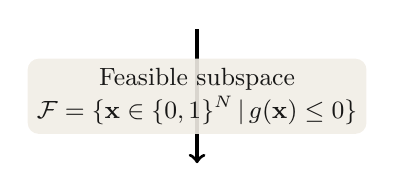
\begin{tikzpicture}
                \draw[very thick,->] (0, 0) -- (0, -1.7);
                \node[align=center, fill=sand, fill opacity=0.9, rounded corners] at (0, -0.85) {\small Feasible
                subspace\\\small $\mathcal{F} = \{\mathbf{x} \in \{0, 1\}^N
                \,|\, g(\mathbf{x}) \leq 0\}$};
            \end{tikzpicture}
            \begin{gather*}
                \mathbf{x}^* = \argmin_\mathbf{x \in \mathcal{F}} f(\mathbf{x})
            \end{gather*}
        \end{block}
    \end{minipage}
\end{frame}

\section{QAOA Brief Introduction}



\begin{frame}{The Quantum Approximate Optimization Ansatz}
\begin{center}
    \begin{itemize}
        \item Variational circuit for combinatorial optimization, introduced
            by~\citeauthor{farhi2014}~\cite{farhi2014}
        \item Trotterization of quantum annealing $H(t) = (1-t) H_M +
            t H_P$
        \item Mixer $H_M = -\sum_{i} \sigma^x_i$, Initial state $\ket{+} = -H_M \ket{+}$
        \item Problem Hamiltonian, e.g. Ising $H_P = -\sum_{i,j} J_{ij} \sigma^z_i
            \sigma_j^z - \sum_i h_i \sigma_i^z$
    \end{itemize}
    \vspace{6pt}
    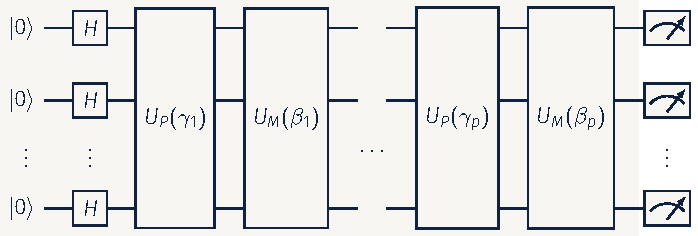
\includegraphics[height=3.0cm]{graphics/build/qaoa.pdf}
\end{center}
\end{frame}

\begin{frame}{Optimization of Parameters}
    \begin{itemize}
        \item State after QAOA iterations $\ket{\beta, \gamma} = \prod_i U_M(\beta_i)
            U_P(\gamma_i) \ket{+}$
        \item Initialize parameters $\beta, \gamma$ with decreasing $\beta$s and
            increasing $\gamma$s
        \item Huge depth $\Rightarrow$ Like QA, $\ket{\beta, \gamma}$ encodes
            good solution already, otherwise
    \end{itemize}
    \begin{block}{Classical training of parameters}
        \[
            \min_{\beta, \gamma} \bra{\beta, \gamma} H_P \ket{\beta, \gamma}
        \]
    \end{block}
\end{frame}

\begin{frame}{The Quantum Alternating Operator Ansatz}
    \begin{itemize}
        \item Generalization of the ansatz by~\citeauthor{hadfield2019}~\cite{hadfield2019}
        \begin{itemize}
            \item $U_P(\gamma)$ \emph{phase-separating} unitary that depends on
                \emph{objective function}
            \item $U_M(\beta)$ \emph{mixing} unitary that depends on
                \emph{domain}
        \end{itemize}
    \end{itemize}
        \begin{block}{Condition for Mixer}
            Map between all feasible states
        \[
            \forall \mathbf{x}, \mathbf{y} \in \mathcal{F},  \exists \beta :
            |\bra{\mathbf{x}}
            U_M(\beta)  \ket{\mathbf{y}}|^2 > 0
        \]
        Do not map between feasible to non-feasible state
        \[
            \forall \mathbf{x} \in \mathcal{F}, \mathbf{y} \notin \mathcal{F},  \forall \beta :
            |\bra{\mathbf{x}}
            U_M(\beta)  \ket{\mathbf{y}}|^2 = 0
        \]
        \end{block}
\end{frame}

\begin{frame}{The Action of the Mixer}
    \centering
    \includegraphics<1>[width=0.8\textwidth]{graphics/build/m_initial.pdf}
    \includegraphics<2>[width=0.8\textwidth]{graphics/build/m_feas_init.pdf}
    \includegraphics<3>[width=0.8\textwidth]{graphics/build/m_feas_no_out.pdf}
    \includegraphics<4>[width=0.8\textwidth]{graphics/build/m_feas_no_out_marked.pdf}
    \includegraphics<5>[width=0.8\textwidth]{graphics/build/m_feas_np.pdf}
    \includegraphics<6>[width=0.8\textwidth]{graphics/build/mixer.pdf}

    \only<5>{Not possible. For unitary reverse way also possible}
\end{frame}


\section{Inequality Constraints so far}

\begin{frame}{Inequality Constraints so far}
    \begin{minipage}{0.5\textwidth}
        To introduce inequality constraints to\\binary optimization
        \begin{itemize}
            \item Slack variables $\mathbf{y} \in \{0, 1\}^M$ that allow range through integer
                encoding
            \item $r_\mathbf{y} = \alpha \sum_m 2^m y_m$ with $\alpha = \min_{\mathbf{x} \in
                \mathcal{F}} g(\mathbf{x})/(2^M - 1)$
            \item $f(\mathbf{x}) \rightarrow f(\mathbf{x}) + \lambda
                (g(\mathbf{x}) - r_\mathbf{y})^2$\\
                assigns large penalties to infeasible states
        \end{itemize}
    \end{minipage}%
    \begin{minipage}{0.5\textwidth}
        \begin{block}{Issues}
            \vspace{10pt}
            \begin{itemize}
                \item Objective function gets distorted\\for values of
                    $g(\mathbf{x})$ that do not fit the grid spanned by
                    $\mathbf{y}$
                \item Potentially large penalty-factor diminishes the objective
                \item Each constraint requires own slack variables
                \item Infeasible states can still be found
            \end{itemize}
        \end{block}
    \end{minipage}
\end{frame}


\begin{frame}{Inequality Constraints so far}
    \centering
    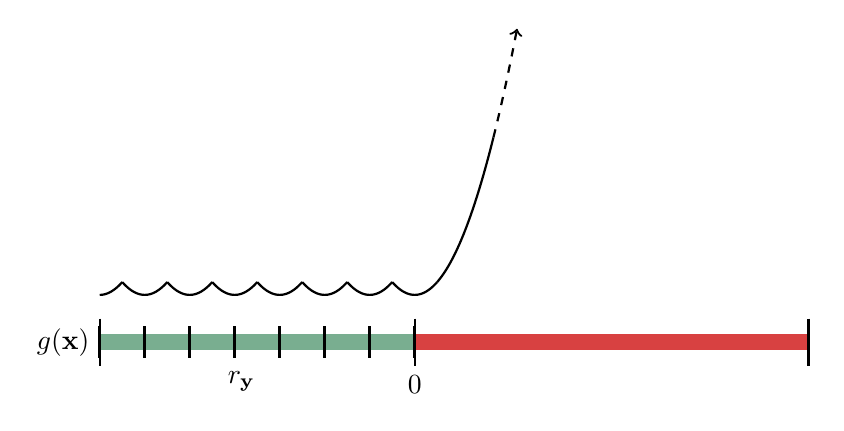
\begin{tikzpicture}
        \draw[color=fire, line width=2mm] (0, 0) -- (5cm, 0);
        \draw[color=success, line width=2mm] (0, 0) -- (-4cm, 0);

        \draw[thick] (0, 0.3) -- (0, -0.3) node[below] {0};
        \draw[thick] (-4cm, 0.3) -- node[left] {$g(\mathbf{x})$} (-4cm, -0.3) ;
        \draw[thick] (5cm, 0.3) -- (5cm, -0.3);

        \foreach \i in {0,...,7} {
            \draw<2->[very thick] (-4cm * \i / 7, 0.2) -- ++(0, -0.4);%
        }
        \foreach \i in {0,...,6} {
            \draw<3>[domain=-0.5714/2:0.5714/2, smooth, variable=\x, thick,
            yshift=0.6cm, xshift=-4cm * \i / 7] plot ({\x}, {2 * \x*\x});%
        }
        \draw<3>[domain=0:0.5714/2, smooth, variable=\x, thick,
            yshift=0.6cm, xshift=-4cm] plot ({\x}, {2 * \x*\x});%
        \draw<3>[domain=0.5714/2:1, smooth, variable=\x, thick,
            yshift=0.6cm] plot ({\x}, {2 * \x*\x});%
        \draw<3>[domain=1:1.3, smooth, variable=\x, thick, dashed, ->,
            yshift=0.6cm] plot ({\x}, {2 * \x*\x});%

        \node<2-> at (-2.2cm, -0.5) {$r_\mathbf{y}$};%
    \end{tikzpicture}
\end{frame}


\section{Constrained Mixer for Inequality Constraints}

\begin{frame}{Phase Mapping}
    \centering
    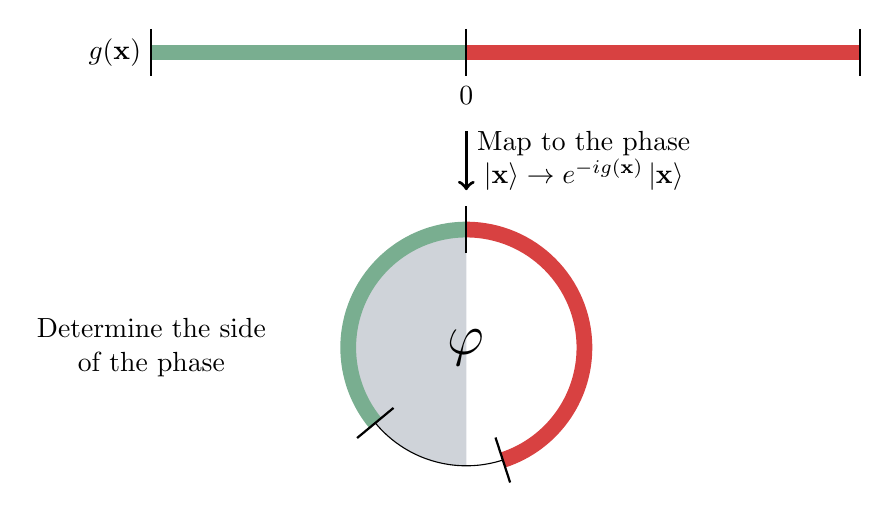
\begin{tikzpicture}
        \draw[color=fire, line width=2mm] (0, 0) -- (5cm, 0);
        \draw[color=success, line width=2mm] (0, 0) -- (-4cm, 0);

        \draw[thick] (0, 0.3) -- (0, -0.3) node[below] {0};
        \draw[thick] (-4cm, 0.3) -- node[left] {$g(\mathbf{x})$} (-4cm, -0.3) ;
        \draw[thick] (5cm, 0.3) -- (5cm, -0.3);

        \draw<2->[->, very thick] (0, -1) -- node[right, align=center] {Map to the
        phase\\$\ket{\mathbf{x}} \rightarrow e^{-i g(\mathbf{x})
        }\ket{\mathbf{x}}$} ++(0, -0.75);

        \fill<3>[color=aqua!20, line width=2mm, yshift=-2.25cm] (0, 0) arc (90:270:1.5cm);
        \draw<2-> (0,-3.75cm) node{\huge $\varphi$} circle (1.5cm);
        \draw<2->[color=fire, line width=2mm, yshift=-2.25cm] (0, 0) arc (90:-72:1.5cm);
        \draw<2->[color=success, line width=2mm, yshift=-2.25cm] (0, 0) arc
        (90:219.6:1.5cm);

        \draw<2->[thick, yshift=-3.75cm] (90:1.2cm) -- (90:1.8cm);
        \draw<2->[thick, yshift=-3.75cm] (-72:1.2cm) -- (-72:1.8cm);
        \draw<2->[thick, yshift=-3.75cm] (219.6:1.2cm) -- (219.6:1.8cm);

        \node<3>[align=center] at (-4cm, -3.75cm) {Determine the side\\of the phase};

    \end{tikzpicture}
\end{frame}

\begin{frame}{Quantum Phase Estimation}
    \begin{minipage}{0.35\textwidth}
        \includegraphics[width=\textwidth]{graphics/build/qpe.pdf}
    \end{minipage}%
    \begin{minipage}{0.65\textwidth}
        \begin{itemize}
            \item Rescale the constraint function, such that $-\pi \leq
                g(\mathbf{x}) \leq \pi$
            \item Measure $\varphi_1$ to determine whether $\varphi = g(\mathbf{x})$ positive or negative.
        \begin{align*}
            P(\varphi \leq 0) = \frac{1}{2^{2M}}\sum_{m = 0}^{2^{(M-1)} - 1}
            \left|\frac{\sin(2\pi m + 2^M\varphi)}{\sin(2^{-M+1}\pi m +
            \varphi)} \right|^2
        \end{align*}
            \item The more ancilla qubits the more $P(\varphi \leq 0)$
                resembles Heaviside theta $\theta(-\varphi)$
        \end{itemize}
    \end{minipage}
\end{frame}

\begin{frame}{Quantum Phase Estimation}
    \centering
    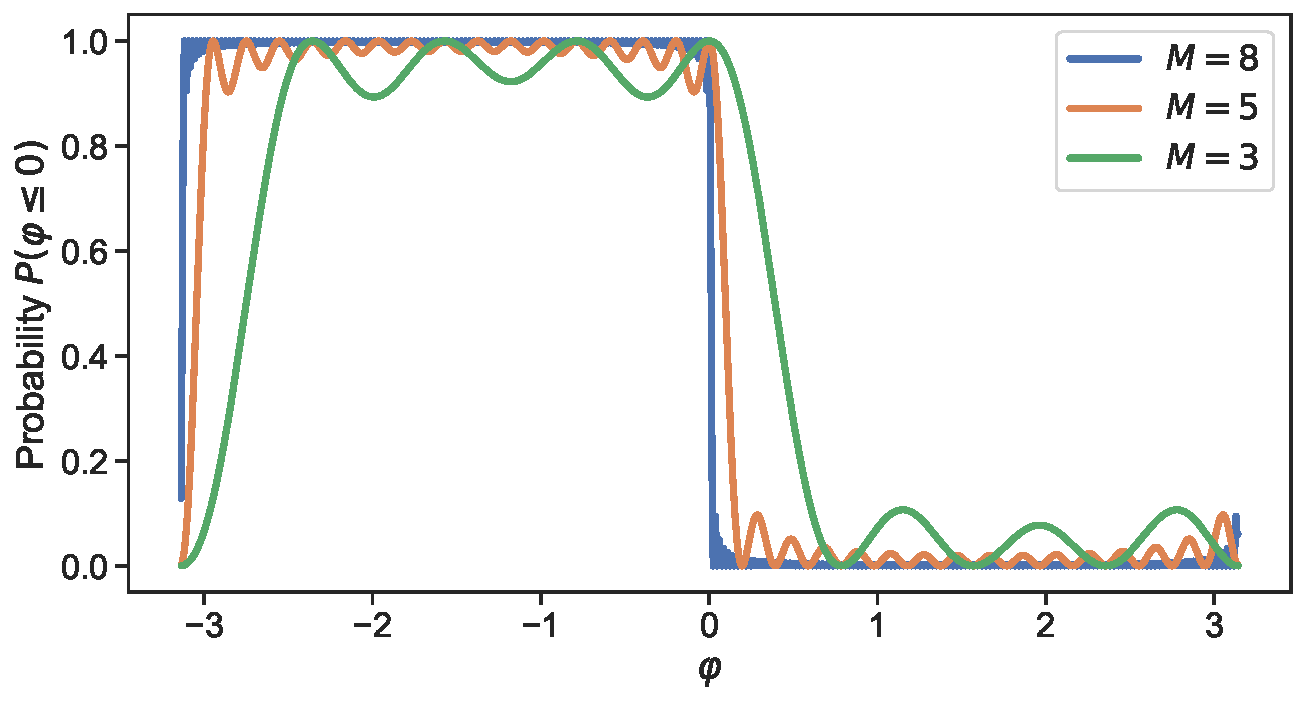
\includegraphics[width=0.88\textwidth]{../plots/prob.pdf}
\end{frame}

\begin{frame}{The new QAOA Layer}
    \includegraphics[width=\textwidth]{graphics/build/cqaoa.pdf}
    \[
        \text{New Mixer operator (not unitary)}\quad \tilde{U}_M(\beta) = \hat P_{g\leq0} \exp \left(-i\beta \sum_i \sigma^x_i\right) 
    \]
    \[
        \forall\mathbf{x} \in \mathcal{F}, \mathbf{y} \notin \mathcal{F}:\quad
        |\bra{\mathbf{y}}\hat P_{g \leq 0} U_M(\beta) \ket{\mathbf{x}}|^2 \leq
        P[g(\mathbf{y}) \leq 0] \xrightarrow{M\rightarrow
    \infty} 0
    \]
\end{frame}

\begin{frame}{A note on success probability}
    \begin{center}
        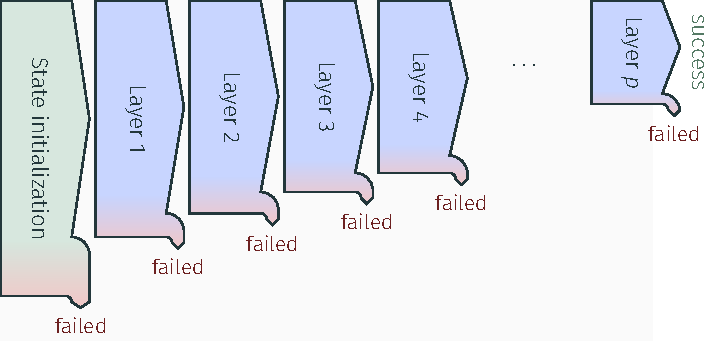
\includegraphics[width=0.65\textwidth]{graphics/build/probability.pdf}
    \end{center}
    Each layer has the chance of succeeding $p_i \Rightarrow$ All layers together
    $p_\text{success} = \prod_i p_i$.
    \[
        p_i = \sum_{\mathbf{x}} |\psi_\mathbf{x}|^2 P[g(\mathbf{x}) \leq 0]
    \]
\end{frame}


\section{Experiments}

\begin{frame}{Simple Example}
    Function $f(x, y)$ of two 4-bit integers. Simple linear inequality
    constraint.
    \begin{center}
        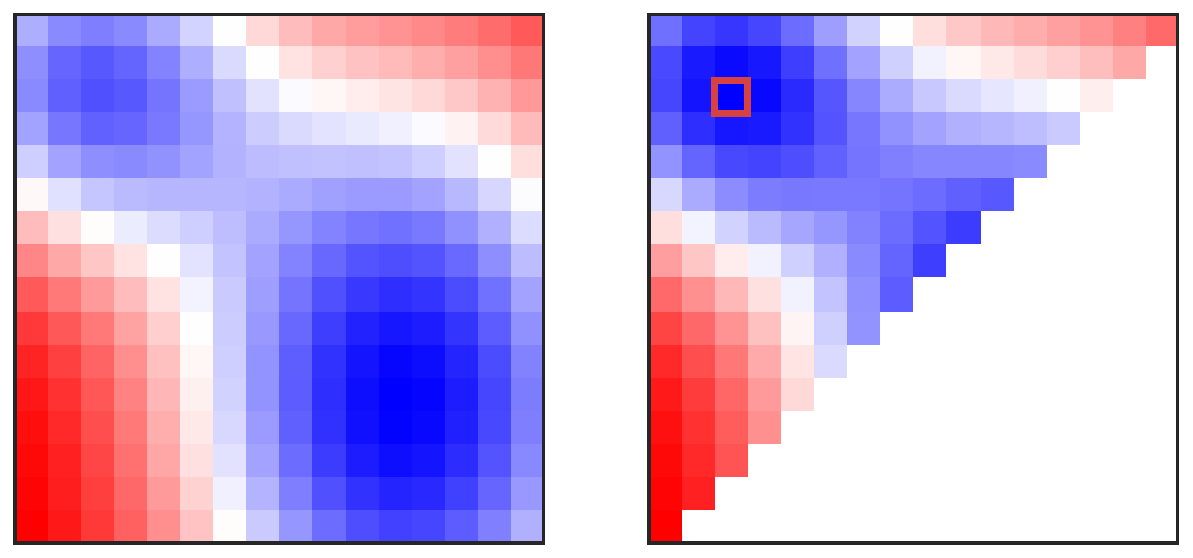
\includegraphics[width=0.7\textwidth]{../plots/example1.pdf}
    \end{center}
\end{frame}

\begin{frame}{Simple Example}
    QPE Method. 500 iterations of Gradient Descent with ADAM.
    \begin{center}
        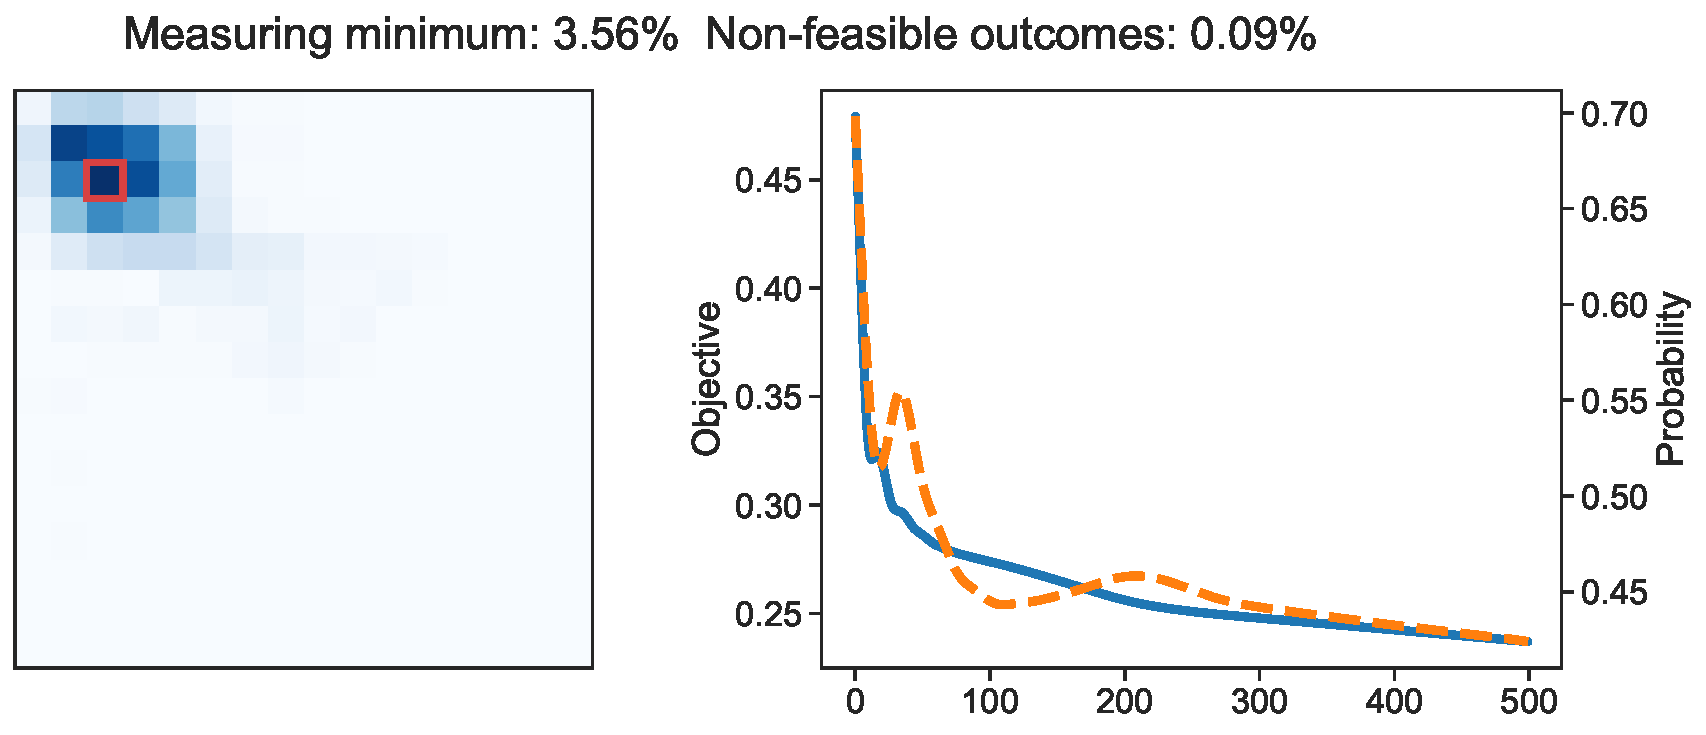
\includegraphics[width=0.9\textwidth]{../plots/opt_example1_masked.pdf}
    \end{center}
\end{frame}

\begin{frame}{Simple Example}
    Penalty Method. 500 iterations of Gradient Descent with ADAM.
    \begin{center}
        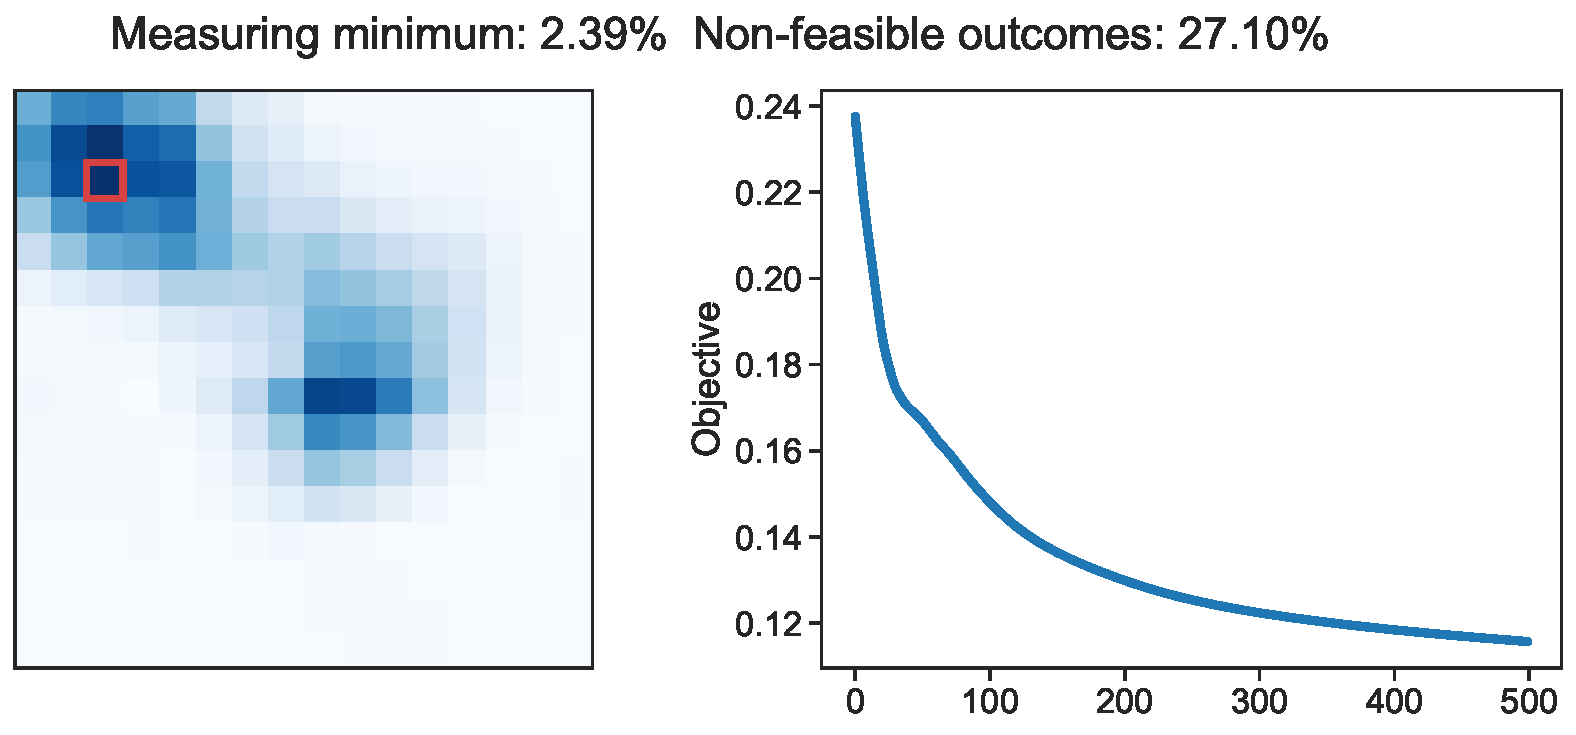
\includegraphics[width=0.9\textwidth]{../plots/opt_example1_penalty.pdf}
    \end{center}
\end{frame}

\begin{frame}{What about the success probability?}
    Quantum Annealing parametrization.
    \begin{center}
        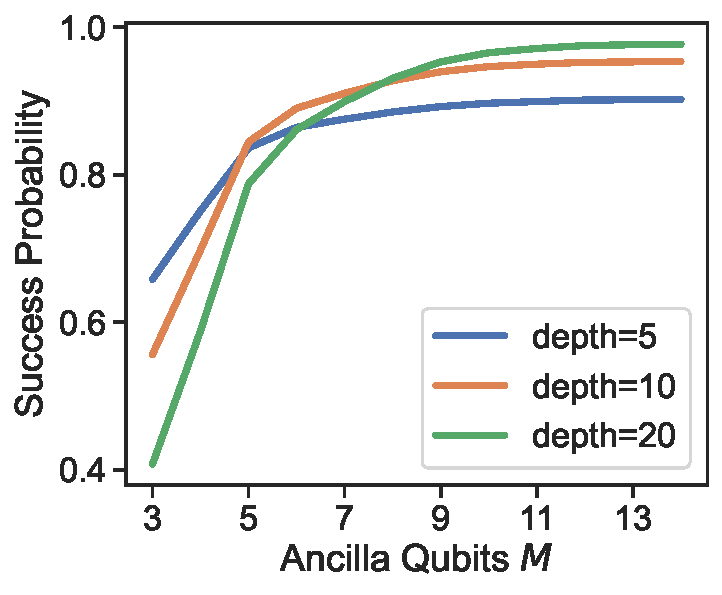
\includegraphics[width=0.45\textwidth]{../plots/prob_num_qubits.pdf}
        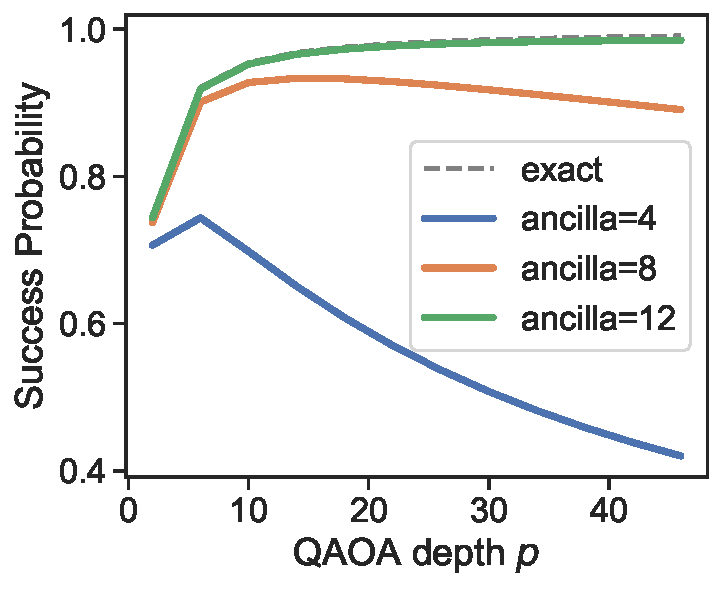
\includegraphics[width=0.45\textwidth]{../plots/prob_depth.pdf}
    \end{center}
\end{frame}

\begin{frame}{A little more complex example}
    \begin{center}
        \includegraphics<1>[width=0.9\textwidth]{../plots/example2.pdf}
        \includegraphics<2>[width=0.9\textwidth]{../plots/opt_example2_masked_12.pdf}
        \includegraphics<3>[width=0.9\textwidth]{../plots/opt_example2_penalty_12.pdf}
    \end{center}
\end{frame}

\section{Conclusion and future directions}

\begin{frame}{Conclusion and future directions}
    \begin{itemize}
        \item Promising first results, but more in depth research needs to be
            conducted
        \item Shrinking success probability is the main caveat
        \item Deeper comparison between the penalty and the QPU based ansätze.
            May have advantage for some kinds of constraints.
        \item Similar ansatz based on Quantum Zeno Dynamics provided advantage
            on real hardware tests~\cite{herman2023}.
    \end{itemize}
\end{frame}

\begin{frame}[allowframebreaks]
    \frametitle{References}
    \printbibliography[heading=none]
\end{frame}

\end{document}
